\chapter{Geophysical Concepts}

This %
\marginelement{Most considerations in this chapter follow two great textbooks by \citeauthorfull{pedloskyoct}: \citebook{pedloskyoct} and \citebook{pedloskygfd}.}%
chapter summarizes some of the physical concepts and mechanisms required to understand the later chapters of my thesis. It touches upon basic geophysical fluid dynamics and describes some of the relevant ocean currents, and is meant as an introduction to Physical Oceanography in general.

In \secref{sec:physics-models}, a set of fundamental equations describing the large-scale flow in the ocean is derived (momentum, continuity, and vorticity equations). Following up, these equations are simplified by making some common assumptions about the dominant processes in the ocean, in order to gain an intuition about the most important mechanisms controlling the ocean circulation, and to establish a solid foundation for later chapters.

\secref{sec:physics-solutions} presents the Sverdrup and Munk solutions to the equations derived before, to showcase how even simple assumptions may lead to powerful descriptions of the ocean, with a wide range of applicability.

\secref{sec:physics-friction} summarizes the role and parameterization of friction in ocean models, introducing the two most common formulations of friction in modeling (diffusive and bottom friction), and reviewing some numerical aspects of a diffusive term (stability and numerical noise).

\secref{sec:physics-currents} contains an introduction to some relevant currents and circulation systems in the real ocean (the global overturning, the \acl{AMOC}, and the \acl{ITF}).
 
\clearpage
\section{Fundamental Models}
\label{sec:physics-models}
Many %
\sidefigure*{Sir George Stokes (1819--1903). \href{https://commons.wikimedia.org/wiki/File:Ggstokes.jpg}{Public Domain}.}{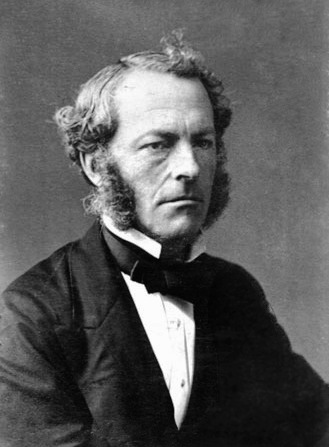
\includegraphics[width=0.9\marginparwidth]{physics/stokes.jpg}}%
different ocean models exist, from highly idealized, qualitative ones, to \acp{GCM} or even coupled Earth System Models with nearly arbitrary complexity. It is neither possible nor feasible to consider every existing dynamics of the ocean during this study. The following sections present three different, common views of the ocean of varying complexity: A general model in three dimensions (\secref{sec:generaleq}), a model retaining only leading-order processes (\secref{sec:leadingorder}), and a simple layered model (\secref{sec:physics-layered}). 

Each of these models is represented by a characteristic set of equations (continuity, momentum, and vorticity equations), and each of these models is useful to gain an intuition of certain sub-processes in the ocean, which will prove to be helpful in later chapters.

\subsection{General Circulations}
\label{sec:generaleq}
This section presents a model that describes a \enquote{general} large-scale circulation, making as few assumptions as necessary (and I am trying to avoid making implicit assumptions in the process).

\subsubsection{Momentum Equations}
Most of modern Physical Oceanography revolves around solving some formulation of the Navier-Stokes Equations for incompressible flow. In their full form, they are still poorly understood, albeit already formulated by George Stokes in 1845 (\cite{joseph}) --- for instance, it has still not been proven that smooth solutions on \(\mathbb{R}^3\) always exist\sidenote[-4]{This has in fact been deemed a \q{Millennium Problem} by the \textsl{Clay Mathematics Institute}, worth a \SI{1000000}[\$]{} cash prize.}. The Navier-Stokes Equations are derived by considering the momentum balance of a fluid parcel, and in vectorial form they read:\sidenote[-1]{See front matter for information on mathematical notation.}
%
\sidedef{Navier-Stokes Equations}{}{%
\begin{align}
\label{eq:navierstokes}
\underbrace{
	\overbrace{
		\frac{\partial}{\partial t}\vec{u}
	}^\text{transient} + \overbrace{
	\left(\vec{u}\cdot\nabla\right)\vec{u} \vphantom{\frac{\partial}{\partial}}
}^\text{advection}
}_\text{material derivative}
- \underbrace{
	\vec{\mathcal{F}}
	\vphantom{\frac{\partial}{\partial}}
}_{\mathclap{\text{dissipation}}}
= 
\overbrace{
	-\frac{1}{\rho} \nabla p
	\vphantom{\frac{\partial}{\partial}}
}^{\mathclap{\text{internal forces}}} \hspace*{1ex}
+ \underbrace{
	\vec{g}
	\vphantom{\frac{\partial}{\partial}}
}_{\mathclap{\text{external forces}}}
\end{align}
}
with
\begin{items}
	\item fluid density \(\rho\);
	\item velocity components \(\vec{u}\);
	\item frictional forces \(\vec{\mathcal{F}}\), often modeled as \(\mu \nabla^2 \vec{u}\) (lateral friction) or \(- \kappa \vec{u}\) (bottom friction)\sidenote[-1]{More on dissipative terms in \secref{sec:physics-friction}.};
	\item pressure \(p\); and
	\item body accelerations \(\vec{g}\).
\end{items}

However, this form of the Navier-Stokes equations is too general to be of practical use in Oceanography. \(\vec{g}\) is actually well-known, since the only relevant body forces in the ocean are gravity and the Coriolis force, hence:
%
\begin{equation} 
\label{eq:bodyforces}
\vec{g} = - 2\vec{\Omega} \times \vec{u} - g \hat{z} 
= \begin{pmatrix} -2\omega(v \sin\theta - w \cos\theta) \\ 2\omega u \sin\theta \\ -2\omega u \cos\theta - g \end{pmatrix}
\end{equation}
%
with
%
\begin{align}
\vec{\Omega} &= \omega (\cos\theta \hat{y} + \sin\theta \hat{z}) & \text{(Earth's angular velocity)} \\
\omega &= \frac{2\pi}{\SI{24}{\hour}} = \SI{7.27e-5}{\per\second}  & \text{(Earth's rate of rotation)} \\
f &= 2 \omega \sin\theta & \text{(Coriolis parameter)} \\
g &= \SI{9.81}{\metre\per\second^2} & \text{(Gravitational acceleration)}
\end{align}

Plugging \eqref{eq:bodyforces} into \eqref{eq:navierstokes} then yields:
%
\sidedef{Momentum Equations}{in vector form}{
\begin{equation}
\vec*{u}{t} + (\vec{u}\cdot\nabla)\vec{u} + 2\vec{\Omega}\times\vec{u} + g\hat{z} = -\frac{1}{\rho} \nabla p + \vec{\mathcal{F}} \label{eq:momentumvec}
\end{equation}
}

\subsubsection{Continuity Equation}
The most fundamental constraint in fluid dynamics that needs to be fulfilled unconditionally by all successful models is mass conservation. It is usually expressed through a continuity equation, describing the evolution of the fluid density \(\rho\) in the flow field:
%
\sidedef{Continuity Equation}{in general form}{
\begin{equation}
\underbrace{\rho_t}_\text{transient} + \underbrace{\nabla \cdot (\rho \vec{u})}_{\mathclap{\text{convection}}} = 
\overbrace{\rho_t + \underbrace{\vec{u} \cdot \nabla \rho}_{\text{advection}}}^{\mathclap{\text{material derivative}}} + \underbrace{\rho \nabla \cdot \vec{u}}_{\mathclap{\text{divergence}}}
 = \underbrace{S(\vec{x},t) \vphantom{\nabla}} _{\mathclap{\text{sources}}}
\label{eq:continuity-general}
\end{equation}
}

In large parts of the ocean, the components adding up to the velocity divergence (\ie \(u_x, v_y, w_z\)) will be much larger than any explicit source or the advection of density. In this case, \eqref{eq:continuity-general} can be decomposed, and each contribution can be required to hold separately:\sidenote[0]{See \citebook{vallis} for a discussion on the validity of this assumption.}
%
\begin{gather}
\nabla \cdot \vec{u} = u_x + v_y + w_z = 0 \vphantom{\Ddx} \label{eq:incompressible} \\
\text{and} \\
\Ddx \rho = S(\vec{x},t) \label{eq:continuity-diabatic}
\end{gather}
%
The first statement is often cited as a condition for an \emph{incompressible fluid}, and holds to a very high degree in the ocean\sidenote[-1]{See \citebook{pedloskywaves}, where Pedlosky derives that gravity waves are divergence-free for phase speeds that are small compared to the speed of sound.}. The second condition describes the evolution of density due to explicit sources, \ie diapycnal (\enquote{cross-isopycnal}) mixing. In an adiabatic ocean,%
\begin{equation} 
	\Ddx \rho = S \equiv 0, \label{eq:adiabatic}
\end{equation}
%
which is a good approximation in the deep ocean.

\subsubsection{Vorticity Equation}
\label{sec:general-vorticity}
Although vorticity is a critical quantity for the large-scale movement of the oceans, it is hard to deal with intuitively, since rotating flows usually do not occur in everyday life. Thus, the most important concepts regarding vorticity (and its conservation) shall be introduced here.

The \emph{relative vorticity} \(\vec{\omega}\) is generally defined as the curl of the velocity field:\sidenote[0]{And is thus a measure for the shear of the flow, and an indicator for its rate of rotation.}
%
\begin{equation}
\vec{\omega} = \nabla \times \vec{u} \label{eq:vorticityvec}
\end{equation}
%
The evolution of vorticity in a system is described by the \emph{vorticity equation}. It can be derived from the 3-dimensional momentum equations in vectorial form, \eqref{eq:momentumvec}. Replacing the advection term \((\vec{u}\cdot\nabla)\vec{u}\) in \eqref{eq:momentumvec} by%
%
\sidenote[-2]{As the vector dot product identity\\[0.5ex]
	 \(\nabla(\vec{a}\cdot\vec{b}) = (\vec{a}\cdot\nabla)\vec{b} + (\vec{b}\cdot\nabla\vec{a}) + \vec{a}\times(\nabla\times\vec{b}) + \vec{b}\times(\nabla\times\vec{a})\)\\[0.5ex]
	with \(\vec{a} = \vec{b} = \vec{u}\) gives\\[0.5ex]
	\(\nabla(|\vec{u}|^2) = 2(\vec{u}\cdot\nabla)\vec{u} - 2(\nabla\times\vec{u})\times\vec{u}\).%
}
%
\begin{equation}
(\vec{u}\cdot\nabla)\vec{u} = \vec{\omega}\times\vec{u} + \nabla\left( \frac{|\vec{u}|^2}{2}\right)
\end{equation}
%
yields
%
\begin{equation}
\vec*{u}{t} + \frac{1}{2} \nabla(|\vec{u}|^2) + (\vec{\omega} + 2\vec{\Omega})\times\vec{u} + g\hat{z} = - \frac{1}{\rho} \nabla p + \vec{\mathcal{F}}. \label{eq:momentumvec2}
\end{equation}
%
Applying the curl operator to \eqref{eq:momentumvec2}, and using that \(\nabla\times\nabla\phi=0\) for any scalar field \(\phi\), leads to
%
\begin{equation} 
\vec*{\omega}{t} + \nabla\times(\vec*{\omega}{a}\times\vec{u}) = \frac{\nabla \rho \times \nabla p}{\rho^2} + \nabla\times\vec{\mathcal{F}} \label{eq:vorticity-1}
\end{equation}
%
with \(\vec*{\omega}{a} = \vec{\omega} + 2\vec{\Omega}\), a quantity called \emph{absolute vorticity}.

This first formulation of the vorticity equation can be simplified further by applying the vector identity
%
\begin{equation}
\nabla\times(\vec*{\omega}{a}\times\vec{u}) = \vec*{\omega}{a}\nabla\cdot\vec{u} + (\vec{u}\cdot\nabla)\vec*{\omega}{a} - \vec{u} \underbrace{\nabla\cdot\vec*{\omega}{a}}_{=0} - (\vec*{\omega}{a}\cdot\nabla)\vec{u}
\end{equation}
%
yielding
%
\sidedef{Vorticity Equation}{in general form}{
\begin{equation}
\underbrace{\Ddx \vec*{\omega}{a}
\vphantom{\frac{D}{\rho^2}}}_{\text{(i)}}
= \underbrace{(\vec*{\omega}{a}\cdot\nabla)\vec{u} \vphantom{\frac{D}{\rho^2}}}_{\text{(ii)}} 
- \underbrace{\vec*{\omega}{a}\nabla\cdot\vec{u} \vphantom{\frac{D}{\rho^2}}}_{\text{(iii)}} 
+ \underbrace{\frac{\nabla \rho \times \nabla p}{\rho^2} \vphantom{\frac{D}{\rho^2}}}_{\text{(iv)}} 
+ \underbrace{\nabla\times\vec{\mathcal{F}} \vphantom{\frac{D}{\rho^2}}}_{\text{(v)}}. 
\label{eq:vorticity-vector}
\end{equation}
}
%
The absolute vorticity \(\vec*{\omega}{a}\) of the flow is thus altered through:
\begin{renum}
\item advection along a streamline;
\item twisting / tilting due to velocity shear;
\item convergence / divergence of the flow (sources / sinks);
\item baroclinic flow; and
\item curl of frictional forces.
\end{renum}

\subsubsection{Potential Vorticity}

The vorticity equation had not been as central as it is in Oceanography without one very important property: the conservation of \ac{PV}. In order to re-formulate \eqref{eq:vorticity-vector} as a conservation law, the continuity equation \eqref{eq:continuity-general} in the form\sidenote[-3]{Assuming the absence of explicit sources, but not necessarily incompressibility.}
%
\begin{equation}
\nabla\cdot\vec{u} = -\frac{1}{\rho} \Ddx[\rho]
\end{equation}
%
is used to eliminate the divergence of the flow from the vorticity equation:
%
\begin{equation}
\Ddx \left( \frac{\vec*{\omega}{a}}{\rho} \right) = \left( \frac{\vec*{\omega}{a}}{\rho} \cdot \nabla \right) \vec{u} + \frac{\nabla\rho\times\nabla p}{\rho^3} + \frac{1}{\rho} \nabla\times\vec{\mathcal{F}} \label{eq:potvort1}
\end{equation}
%
Multiplying \eqref{eq:potvort1} with a scalar fluid property \(\lambda\) that fulfills the condition
%
\begin{equation}
\Ddx[\lambda] = \Lambda
\end{equation}
%
with some unspecified source \(\Lambda\), ultimately leads to\sidenote{See \citebook{pedloskygfd}.}
%
\begin{equation}
\label{eq:pv-conservation}
\Ddx \Pi = 
\underbrace{\frac{\vec*{\omega}{a}}{\rho} \cdot \nabla \Lambda \vphantom{\frac{\nabla}{\rho^3}}}_{\substack{\text{sources}\\\text{(i)}}}
+ \underbrace{\nabla \lambda \cdot \left( \frac{\nabla p \times \nabla \rho}{\rho^3}\right)}_{\substack{\text{baroclinity}\\\text{(ii)}}}
+ \underbrace{\frac{\nabla\lambda}{\rho} \cdot \left(\nabla\times\vec{\mathcal{F}}\right)}_{\substack{\text{friction}\\\text{(iii)}}}
\end{equation}
%
where \(\Pi\) is called \emph{potential vorticity}:
%
\sidedef{Potential Vorticity}{in general form}{
\begin{equation}
\Pi = \frac{\vec*{\omega}{a}}{\rho} \cdot \nabla \lambda \label{eq:potvort}
\end{equation}
}
%
Equation \ref{eq:pv-conservation} thus implies that potential vorticity is a \emph{conserved quantity} if the following conditions are fulfilled:
\begin{renum}
	\item \(\lambda\) is conserved along streamlines, \ie \(\Lambda = 0\);
	\item frictional forcing is negligible (\(\vec{\mathcal{F}} \approx 0\)); and
	\item the flow is purely barotropic, \ie \(\nabla p \times \nabla \rho = 0\); \emph{or} \(\lambda \equiv \lambda(p,\rho)\), \ie \(\lambda\) is a function of pressure and density alone.\sidenote[-1]{\(\nabla\lambda(p,\rho) = \lambda_\rho \nabla \rho + \lambda_p \nabla p\), \(\rightarrow \nabla \lambda \cdot (\nabla p \times \nabla \rho) = 0\), a fundamental property of the box product.}
\end{renum} 
%
One possible, natural choice for \(\lambda\) in the ocean is density, \ie \(\lambda \equiv \rho\). The first condition is then valid for purely adiabatic flow by definition \eqref{eq:adiabatic}, and the third condition is fulfilled unconditionally (since \(\lambda\) then trivially depends on \(\rho\) only). Hence, \(\Pi_{\lambda = \rho} = \vec*{\omega}{a} / \rho \cdot \nabla \rho\) is conserved in the absence of friction and diapycnal mixing.

\parabreak

The conservation of potential vorticity is one of the most powerful constraints in all of Oceanography. Since frictional forces and diabatic processes are typically negligible in the interior ocean, a solution for the large-scale interior circulation can directly be inferred from the vorticity equation (the Sverdrup solution, \cf \secref{sec:sverdrup}).

\subsection{Leading-Order Equations}
\label{sec:leadingorder}
While \secref{sec:generaleq} introduces a set of equations that describe nearly every possible ocean dynamics, it is often useful to approximate the general equations using some reasonable assumptions in order to reduce the complexity of the system. This is in fact one of the most common approaches in Oceanography: Since, on one hand, the general equations of motion (momentum equations plus continuity equation) are mathematically very difficult to treat\sidenote[-3]{Four three-dimensional, nonlinear, coupled partial differential equations, thus allowing for chaotic behavior in the form of turbulence.}, and, on the other hand, the observed behavior of the ocean is pretty simple in most regions (mostly linear, two-dimensional flow), there is an inherent need for finding sensible approximations.

In this section, some approximations that are suitable in a large portion of the ocean are applied to retain a simpler set of equations --- namely:
\begin{items}
	\item the small aspect ratio of the ocean, suppressing vertical terms;
	\item the Boussinesq Approximation;
	\item hydrostatic balance; and
	\item geostrophic balance as leading-order dynamics.
\end{items}

\subsubsection{Momentum \& Continuity Equations}
For large-scale circulations in the open ocean, horizontal length scales \(L\) are typically much larger than the vertical length scale \(D\). Reasonable scales for the Atlantic Ocean would be \(L = \SI{5000}{\kilo\metre}\) and \(D = \SI{5}{\kilo\metre}\), giving an aspect ratio \(\delta\) of about \(\delta = \frac{D}{L} \approx 10^{-3} \ll 1\).  This leads to the assumption that 
%
\begin{equation}
\orderof{w} = \frac{D}{T} \ll \orderof{u} = \frac{L}{T} \label{eq:wsmall}
\end{equation}
%
with a typical time scale \(T\). An approximate form of the body forcing \(\vec{g}\) in the Navier-Stokes equations \eqref{eq:navierstokes} is thus\sidenote[-1]{Also assuming that\linebreak
\(\orderof{2\omega u \cos\theta} = \SI{1.5e-4}{\per\second} u \ll g\).}:
%
\begin{equation}
\vec{g} = \begin{pmatrix} - f(v - w \cot\theta) \\ fu \\ -fu\cot\theta - g \end{pmatrix} \approx \begin{pmatrix} -fv \\ fu \\ -g \end{pmatrix} \label{eq:approxbodyforces}
\end{equation}
%
Plugging \eqref{eq:approxbodyforces} into \eqref{eq:navierstokes} then yields
%
\begin{align}
u_t + u u_x + v u_y + w u_z - fv &= -\frac{p_x}{\rho} + \hat{x} \cdot \vec{\mathcal{F}} \nonumber \\
v_t + u v_x + v v_y + w v_z + fu &= -\frac{p_y}{\rho} + \hat{y} \cdot \vec{\mathcal{F}}
\label{eq:approxmomentum}\\
w_t + u w_x + v w_y + w w_z + g &= -\frac{p_z}{\rho} + \hat{z} \cdot \vec{\mathcal{F}}. \nonumber
\end{align}
%
A sensible decomposition of \(p\) and \(\rho\) into a static background value and one influenced by the flow field (\(\rho_0(z)\) and \(\rho'(x,y,z)\), respectively) leads to the insight that the leading-order balance in the horizontal momentum equations must be\sidenote[0]{This is shown \eg in \citebook{pedloskygfd}.}
%
\begin{align}
fv &= \frac{1}{\rho_0} p'_x \\
fu &= -\frac{1}{\rho_0} p'_y \label{eq:geostrophy}
\end{align}
%
which is called \emph{geostrophic balance} (whereas replacing \(\rho\) with \(\rho_0\) is called the \emph{Boussinesq Approximation}). Using the same argument, the \(w\)-equation becomes to a good approximation
%
\begin{equation}
p_z = -\rho g, \label{eq:hydrostatic}
\end{equation}
%
which is the \emph{hydrostatic balance}.

Plugging \eqref{eq:geostrophy} into the continuity equation for incompressible flow \eqref{eq:incompressible} yields
%
\begin{align}
0 &= \nabla \cdot \vec{u} = - \left( \frac{p'_y}{f\rho_0} \right)_x + \left( \frac{p'_x}{f\rho_0} \right)_y + w_z = \\
&= - \frac{p'_{xy}}{f\rho_0} + \frac{p'_{xy}}{f\rho_0} - \frac{p'_x f_y}{f^2 \rho_0} + w_z.
\end{align}
%
Since
%
\begin{equation}
\orderof{\frac{p'_{xy}}{f \rho_0}} = \frac{U}{L} \quad \text{and} \quad \orderof{\frac{p'_x f_y}{f^2 \rho_0}} = \frac{U}{R_E},
\end{equation}
%
the dominant balance in the continuity equation for flow of a scale \(L\) for which \(L/R_E < 1\) is between the geostrophic terms, which cancel each other. Thus, for flow of scale \(L\), \(w_z \approx 0\) to a leading order. As \(w\) must vanish at flat boundary surfaces, this implies that\sidenote[-3]{A similar result can be obtained from the vorticity equation by assuming linear, inviscid, purely barotropic flow --- this is known as the Taylor-Proudman Theorem.}
%
\begin{equation}
w \approx 0 \label{eq:continuityhor}
\end{equation}
%
for geostrophic flow. Hence, the leading-order momentum equations become in this case
%
\begin{align}
u_t + uu_x + vu_y - fv &= -\frac{p_x}{\rho_0} + \hat{x} \cdot \vec{\mathcal{F}} \\
v_t + uv_x + vv_y + fu &= - \frac{p_y}{\rho_0} + \hat{y} \cdot \vec{\mathcal{F}} \label{eq:momentum-leading} \\
-\rho g &= p_z.
\end{align}

\subsubsection{Stream functions}
According to the fundamental theorem of vector calculus, every (mathematically sane) vector field can be decomposed into two parts, one irrotational (curl-free) and one solenoidal (divergence-free). In three dimensions, the Helmholtz decomposition of the (vector) flow field \(\vec{u}\) is given by
%
\begin{equation}
\vec{u} = - \nabla \Phi + \nabla \times \vec{\Psi}
\end{equation}
%
with a scalar potential \(\Phi\) and a vector potential \(\vec{\Psi}\). In the two-dimensional case (Helmholtz-Hodge decomposition\sidenote[-1]{For a review of the Helmholtz-Hodge decomposition see \eg \cite{bhatia}.}), both of these parts are expressed through a scalar function: the velocity potential \(\Phi\) (irrotational) and the stream function \(\Psi\) (solenoidal), such that
% 
\begin{equation}
\begin{pmatrix} u \\ v \end{pmatrix} = \nabla \Phi + J \nabla \Psi
\end{equation}
%
with
%
\begin{equation}
J = \begin{pmatrix} 0 & -1 \\ 1 & 0 \end{pmatrix},
\end{equation}
%
an operator rotating a 2-dimensional vector counterclockwise by \(\pi/2\). 
Since the leading-order flow is purely horizontal and divergence-free (\cf \eqref{eq:continuityhor}), implying \(\Phi \approx 0\), it can be described by a stream function \(\Psi\) only, with
%
\begin{equation}
Hu = - \Psi_y, \quad Hv = \Psi_x. \label{eq:streamfunc}
\end{equation}
%
Here, \(H\) denotes the total height of the water column, which was added to make sure that \(\Psi\) carries the dimension of a volume transport (\(\si{\cubic\metre\per\second}\), usually measured in Sverdrup: \(\SI{1}{\sv} = \SI{e6}{\cubic\metre\per\second}\)).

A useful property of the stream function stems from the fundamental theorem of calculus for line integrals, which reads
%
\begin{equation}
\Psi(\vec{q}) - \Psi(\vec{p}) = \int_{\gamma} \nabla \Psi(\vec{r})\cdot\dx{\vec{r}} \simeq \int_{\gamma} (V \dx{x} - U \dx{y})
\end{equation}
%
with \(\gamma\) denoting an arbitrary path between the points \(\vec{q}\) and \(\vec{p}\). This essentially implies that the difference of the stream function at two different locations gives the net volume flux through any path connecting them. 

\subsubsection{Vorticity Equation}
With the approximations made so far, the general vorticity equation \eqref{eq:vorticity-vector} can be simplified substantially. First of all, only the vertical component of \(\vec*{\omega}{a}\) is of real interest in leading-order dynamics, \ie when neglecting vertical motion (since \(\hat{x}\cdot\vec{\omega} = w_y - v_z \approx 0\), and equivalently for \(\hat{y}\cdot\vec{\omega}\)). The vertical component of \(\vec{\omega}\) is often referred to as \emph{the} relative vorticity, and denoted as \(\zeta\):
%
 \sidedef{Relative vorticity}{for horizontal flow}{
\begin{equation}
\zeta := \nabla_H \times \vec{u} = v_x - u_y. \label{eq:relvort}
\end{equation}
}
%
The vertical component of the vorticity equation \eqref{eq:vorticity-vector}, as obtained from the leading-order momentum equations as in \eqref{eq:momentum-leading}\sidenote[-1]{This eliminates the baroclinic and tilting terms.}, thus reads
%
\begin{equation}
\Ddx (\zeta + f) + (f + \zeta) \nabla_H \cdot \vec{u} = \nabla_H \times \vec{\mathcal{F}}. \label{eq:vort1}
\end{equation}
%
Replacing the divergence term \(\nabla_H \cdot \vec{u}\) via the continuity equation for incompressible flow, \eqref{eq:incompressible}, \eqref{eq:vort1} can be written as
%
\sidedef{Vorticity Equation}{for horizontal flow}{
\begin{equation}
\Ddx (\zeta + f) = (\zeta + f)w_z + \nabla_H \times \vec{\mathcal{F}}. \label{eq:vorticity-hor}
\end{equation}
}
%
In this case, the horizontal flow is \emph{not} non-divergent, but instead introduces the term \(w_z\) into the vorticity equation. This is justified when realizing that the term \((\zeta + f)\nabla_H \cdot \vec{u}\) involves velocities of a higher order than the ones in geostrophic balance --- the vorticity equation for \emph{purely} geostrophic flow would simply read \(\text{D}/\text{d}t(\zeta + f) = 0\), which could hardly lead to any interesting dynamics.

\subsection{Layered Model}
\label{sec:physics-layered}
Consider an adiabatic\sidenote{In the sense that no diapycnal mixing occurs, \ie surfaces of constant density stay strictly separated with no flow between them.} ocean model with \(n\) layers, each of height \(h_n = z_{n-1} - z_{n}\) and constant density \(\rho_n\), in which the vertical length scale is much smaller than the horizontal. These assumptions, and the insights obtained from the leading-order dynamics described in \secref{sec:leadingorder}, lead to a powerful approximation of the real ocean dynamics.

\subsubsection{Momentum \& Continuity Equations}
Starting %
\sidefigure*{Structure of the layered model}{\import{figures/physics/}{layers.pdf_tex}}[-2]%
with hydrostatic balance \eqref{eq:hydrostatic}, \ie
%
\begin{equation}
p_z = -\rho g,
\end{equation}
%
an expression for the pressure \(p_n\) in the \(n\)-th layer can be obtained:
%
\begin{equation}
p_n = -\rho_n g (z - z_n) - \sum_{i=1}^{n-1} \rho_i g h_i. \label{eq:pres-layer}
\end{equation}
%
This can be rewritten using a dynamic pressure \(\pi\), which only depends on the current stratification:
%
\begin{equation}
p_n = -\rho_n g z + \rho_0 \pi(x,y,t)
\end{equation}
%
with the average (background) density \(\rho_0\).
This expression for \(p_n\) implies that the terms \(p_x\) and \(p_y\) appearing in the horizontal momentum equations cannot depend on \(z\) inside a particular layer. Hence, it makes sense that the horizontal velocities themselves are independent of \(z\), \ie \(u_z = v_z \approx 0\), leading to the same structure of the horizontal momentum equations already found in \secref{sec:leadingorder} (applied to each layer):
%
\begin{align}
u_t + uu_x + vu_y - fv &= -\frac{(p_n)_x}{\rho_0} + \hat{x} \cdot \vec{\mathcal{F}} \\
v_t + uv_x + vv_y + fu &= - \frac{(p_n)_y}{\rho_0} + \hat{y} \cdot \vec{\mathcal{F}}.
\end{align}

In the special case of a two-layer ocean, \eqref{eq:pres-layer} implies
%
\begin{align}
p_1(z) &= -\rho_1 g (z-z_0) \\
p_2(z) &= -\rho_2 g (z-z_1) - \rho_1 g h_1.
\end{align}
%
For the lower layer, this means that the pressure terms in the momentum equation \eqref{eq:momentumvec} take on the form
%
\begin{equation}
-\frac{(p_2)_x}{\rho_0} = \frac{g}{\rho_0} (\rho_1 (h_1)_x + \rho_2 (z_1)_x) \approx \frac{g (\rho_2 - \rho_1)}{\rho_0} (h_1)_x =: \gamma (h_1)_x,
\end{equation}
using the assumption that displacements of the surface \(z_0\) are small compared to the interfacial displacement\sidenote[-1]{This is often refered to as the \emph{rigid lid} condition.} \(z_1\), and hence \((h_1)_x \approx -(z_1)_x\). The so-defined parameter \(\gamma\) is called \emph{reduced gravity} and is of the order \(\SI{0.01}{\metre\per\second\squared}\), since horizontal density variations in the ocean are usually negligible. This retroactively justifies the assumption that interfacial displacements are much larger than those of the surface, since interfacial displacements only need to overcome a much smaller restoring force (\(\gamma\) instead of \(g\)). This is a direct consequence of buoyancy that acts to greatly reduce the effect of gravity on interfacial displacements when density differences are small.

What is remaining is an expression for the evolution of the layer heights \(h_n\). By integrating the continuity equation over a layer we get:\sidenote[-1]{Recall that neither \(u\) nor \(v\) depends on \(z\).}
%
\begin{equation}
0 = \int_{z_{n}}^{z_{n-1}} \nabla \cdot \vec{u} \dx{z} = h_nu_x + h_nv_y + w(z_{n-1}) - w(z_n). \label{eq:contint}
\end{equation}
%
Since there cannot be any flow across the interface boundaries, a kinematic boundary condition must be fulfilled:
%
\begin{equation}
w = \Ddx z \rightarrow \lim_{z \to z_n} w \overset{!}{=} \Ddx z_n.
\end{equation}
%
This essentially says that the change of depth of a particle along a stream line close to the interface must be the same as the change of the depth of the interface itself (which is of course not the case for cross-interfacial flow). The boundary terms involving \(w\) can thus be rewritten as
%
\begin{align}
w(z_n) &= (z_n)_t + u(h_n)_x + v(h_n)_y \\
w(z_{n-1}) &= (z_{n-1})_t + u(h_{n-1})_x + v(h_{n-1})_y,
\label{eq:wbottom} 
\end{align}
%
leading to, assuming \(u(z) \equiv u\), \(v(z) \equiv v\):
%
\sidedef{Continuity Equation}{for the layered model}{
\begin{align}
0 &= h_n(u_x + v_y) + (z_{n-1} - z_n)_t + u (z_{n-1} - z_n)_x + v (z_{n-1} - z_n)_y \\ 
& = (h_n)_t + h_n \nabla_H \cdot \vec{u} + \vec{u} \cdot \nabla_H h_n \\
& = \Ddx h_n + h_n \nabla_H \cdot \vec{u}, \label{eq:continuity-height}
\end{align}
}
%
which is the desired equation describing the evolution of the layer height.

\parabreak

Note that the surface and bottom terms in \eqref{eq:contint} can be neglected entirely if
%
\begin{equation}
\frac{\orderof{w_b}}{\orderof{hu_x}} = \frac{U E / L}{U H / L} = \frac{E}{H} \ll 1
\label{eq:quasigeostrophic}
\end{equation}
%
with \(E\) denoting a typical scale of the \emph{layer height anomaly} \(\eta\) \ie the deviation of \(h\) from an undisturbed layer height \(H\). To put \eqref{eq:quasigeostrophic} into words: If the fluctuations in layer height are small compared to the mean height of the layer, the boundary terms in the integrated continuity equation \eqref{eq:contint} vanish, and the horizontal flow becomes divergence-free. It can then be expressed through a stream function
%
\begin{equation}
U = \int_{z_{n}}^{z_{n-1}} u \dx{z} = -\Psi_y, \quad V = \int_{z_{n}}^{z_{n-1}} v \dx{z} = \Psi_x.
\end{equation}
%
Flow fulfilling the condition posed by \eqref{eq:quasigeostrophic} is called \emph{quasi-geostrophic}, which is obviously the case when integrating over the entire depth of the ocean (this even holds if \(u\) and \(v\) depend on \(z\)).

\subsubsection{Vorticity Equation \oldand Potential Vorticity}
Since the momentum equations for the layered model are of the same form as for the leading-order model described in \secref{sec:leadingorder}, the vorticity equation must also be of a similar form. Replacing \(\nabla_H \cdot \vec{u}\) in \eqref{eq:vort1} by the corresponding term given in \eqref{eq:continuity-height} gives
%
\begin{equation}
\Ddx(\zeta + f) = - \frac{\zeta + f}{h_n}\Ddx[h_n] + \nabla_H \times \vec{\mathcal{F}}, \label{eq:vorticity-layer}
\end{equation}
%
which is equivalent to
%
\begin{equation}
\Ddx\left( \frac{\zeta + f}{h_n} \right) = \frac{1}{h_n} \nabla_H \times \vec{\mathcal{F}}. \label{eq:pv-conservation-layer}
\end{equation}
%
Hence, the \emph{potential vorticity} \(\Pi_s\) is in this case
%
\sidedef{Potential Vorticity}{in a layered ocean}{
\begin{equation}
\Pi_s = \frac{\zeta + f}{h_n}, \label{eq:pv-layer}
\end{equation}
}
%
which differs from the general form of the \ac{PV} only by a constant factor (\(\rho\)). In fact, \eqref{eq:pv-layer} is probably the most frequently used formulation of potential vorticity, at least for mostly horizontal flow. It is extremely useful because its evolution, as given by \eqref{eq:pv-conservation-layer}, reveals the dominant mechanisms behind the large-scale circulation in a layered ocean: As water flows in meridional direction (\ie towards a different \(f\)), the water column can either adjust by assuming a relative rotation (\(\zeta\)), by squeezing or stretching of the entire layer (\(h_n\)), or by dumping excess vorticity through friction (\(\vec{\mathcal{F}}\)).


\section{Notable Solutions}
\label{sec:physics-solutions}
Under certain assumptions, the model equations presented in the previous sections can be solved analytically, yielding solutions for the ocean circulation that are good approximations in large regions of the ocean. Two such solutions are discussed in this section: The Sverdrup solution for the ocean interior, and the Munk solution for a frictional western boundary current.

\subsection{Sverdrup Theory}
\label{sec:sverdrup}
Considering a linear, frictionless, steady, homogeneous ocean forced by wind stress only leads to a powerful theory for the interior ocean circulation, called Sverdrup Theory, which was introduced in \cite{sverdrup}, and is covered in depth in \cite{pedloskyoct}. It is a depth-integrated form of the vorticity equation \eqref{eq:vorticity-hor}, using the following key assumptions\sidenote[-2]{Leading to a balance between advection of planetary vorticity and curl of frictional forces (in this case wind stress).}:

\begin{items}
	\item A low Rossby number \(R_0\), \ie the condition that nonlinear terms are negligible in comparison to the Coriolis term (and thus the geostrophic balance):
	\begin{equation}
	R_0 = \orderof{\frac{\vec{u}\cdot\nabla u}{fv}} = \frac{U^2/L}{fU} = \frac{U}{fL} \ll 1,
	\end{equation}
	with a typical velocity scale \(U\) and horizontal length scale \(L\).
	\item A low horizontal Ekman number \(E_H\), \ie the condition that diffusive terms are negligible in comparison to geostrophy:
	\begin{equation} E_H = \orderof{\frac{A_H \nabla^2 u}{fv}} = \frac{A_H U/L^2}{fU} = \frac{A_H}{fL^2} \ll 1, \end{equation}
	with a horizontal turbulent diffusion constant \(A_H\).
\end{items}
%
Typical values in the interior ocean would be \(U \approx \SI{1}{\cm\per\second}\), \(L \approx \SI{1000}{\kilo\metre}\), \(f \approx \SI{e-4}{\per\second}\), and \(A_H \approx \SI{e-4}{\square\metre\per\second}\) (as found in eddy-resolving models \eg by \cite{bryan}), leading to both \(R_0 \approx 10^{-4}\) and \(E_H \approx 10^{-4}\).

With these assumptions, the famous Sverdrup relation connects the horizontal stream function \(\Psi\) of the vertically integrated flow to the surface wind stress \(\vec{\tau}\) alone:
%
\sidedef{Sverdrup relation}{in spherical coordinates}{
\begin{equation}
\Psi = \frac{-1}{\rho_0 \beta} \int_{\phi}^{\phi_E} \curl(\vec{\tau}) R_E \cos\theta \dx{\phi'} \label{eq:sverdrup}
\end{equation}
}
%
with
%
\begin{items}
	\item the Earth's radius \(R_E \approx \SI{6371}{\kilo\metre}\);
	\item the Coriolis parameter \(\beta = \frac{\omega}{R_E} \cos\theta \approx f_y\);
	\item the latitude of the nearest eastern boundary \(\phi_E\); and
	\item the curl of the horizontal wind stress \(\vec{\tau}\), in spherical coordinates:
	\begin{equation}\curl(\vec{\tau}) = \frac{1}{R_E \cos\theta} \left( -(\hat{x} \cdot \vec{\tau} \cos\theta)_\theta + (\hat{y} \cdot \vec{\tau})_\phi \right).\end{equation}
\end{items}

\subsubsection{Validity of the Sverdrup Relation}
Even though Sverdrup theory is a drastic simplification of the real ocean, it leads to a realistic interior circulation in the subtropical gyres (\figref{fig:sverdrup}), which is why it is of such importance in Physical Oceanography. However, it does not lead to a closed circulation at the western boundary, since the winds have no notable zonal structure (and thus, the value of \(\Psi\) depends mostly on the distance to the eastern boundary). 

This%
%
\sidefigure[Comparison between Sverdrup and barotropic stream functions.]{Sverdrup theory as a first approximation of the ocean circulation. Shown is the transport in Sverdrups (\(\SI{1}{\sv} = \SI{e6}{\cubic\metre\per\second}\)), estimated using \eqref{eq:sverdrup} (top) and the \ac{BSF} (bottom). Data from \ac{CESM} model output.}[fig:sverdrup]%
{\importpgf{figures/physics/sverdrup-comp/}{sverdrup-comp.pgf}}[-3]%
%
implies that effects that have been neglected in Sverdrup theory must be dominant near the western boundaries. This is also directly evident from \eqref{eq:sverdrup}: Since the equation for \(\Psi\) is first order in \(\phi\), it cannot satisfy a no-normal-flow boundary condition at the eastern and western edges of the basin at the same time.

\subsection{Western Boundary Currents} 
The most common approach to tackle this inconsistency of Sverdrup theory is to assume a western boundary layer that is dominated by dynamics that have been neglected in the interior, and smoothly joins the Sverdrup interior solution given by \eqref{eq:sverdrup} for large distances from the western boundary.

Dramatically%
\sidefigure[Location, scale and magnitude of the Kuroshio.]{Location, scale and magnitude of the Kuroshio in the \ang{1} \ac{CESM} default run.}[fig:kuroshio]{%
	\importpgf{figures/physics/kuroshio/}{kuroshio.pgf}
}[8]%
changed length and velocity scales have to be taken into account when dealing with western boundary currents. One real-world example for such a current is the Kuroshio (\figref{fig:kuroshio}), which is located in the North Pacific (analogous to the Gulf Stream in the North Atlantic). \cite{liu} give a width of the Kuroshio of about \(\SI{200}{\kilo\metre}\), and an along-stream mean velocity of about \(\SI{35}{\centi\metre\per\second}\). Thus, both Rossby and horizontal Ekman numbers can safely be assumed to be several magnitudes larger at the western boundary, and any successful theory must include the terms that have been neglected during the derivation of the Sverdrup relation.

\subsubsection{The Munk Boundary Layer}
\label{sec:munk}
One simple solution for the western boundary was published in \cite{munk}. It assumes a linear ocean (\ie a low Rossby number), but includes a frictional term of the form
%
\begin{equation}
\vec{\mathcal{F}} = A_H \nabla^2 \vec{u}
\end{equation}
%
with a constant diffusion coefficient \(A_H\). This leads to
%
\begin{equation}
\curl(\vec{\mathcal{F}}) = A_H \nabla^2 (v_x - u_y) = A_H \nabla^2 \zeta = A_H \nabla^4 \Psi, \label{eq:fricdiff}
\end{equation}
%
where \(\nabla^4\) denotes the biharmonic differential operator such that
%
\begin{equation}
\nabla^4 \Psi = \Psi_{xxxx} + 2 \Psi_{xxyy} + \Psi_{yyyy}.
\end{equation}

As already stated, \citeauthor{munk} assumed a linear boundary layer, hence dropping all nonlinear terms. Also, for the sake of simplicity, he assumed a strictly meridional boundary current, with a zonal length scale \(L_x\) that is much smaller than the meridional length scale \(L_y\) (\ie, a narrow boundary current connecting North and South), leading to the assumption that \(\Psi_x \gg \Psi_y\). A steady-state solution can then be found from the vorticity equation \eqref{eq:vorticity-hor}, retaining only the dominant balance between Coriolis force\sidenote[-1]{Assuming a so-called \(\beta\)-plane, \ie \(f \approx f_0 + \beta y \to f_y \approx \beta\).} and frictional forces:
%
\begin{equation}
\beta \Psi_x = A_H\Psi_{xxxx}. \label{eq:munkode}
\end{equation}
%
At the boundaries, it is required that \(\lim\limits_{x \to 0} \Psi(x) = 0\) and \(\lim\limits_{x \to \infty}\Psi(x) = \Psi_I (x,y)\), with \(\Psi_I\) being the Sverdrup interior solution as in \eqref{eq:sverdrup}. The fourth-order \ac{ODE} \eqref{eq:munkode} is then solved by
%
\sidedef{Munk's solution}{}{
\vskip\baselineskip% looks a little crammed
\begin{equation}
\Psi = \Psi_I(x,y) \Big[ 1-e^{-x/(2\delta_M)} \cos\Big( \frac{\sqrt{3}x}{2\delta_M} \Big) \Big] + C(y) e^{-x/(2\delta_M)} \sin\Big( \frac{\sqrt{3}x}{2\delta_M} \Big),
\end{equation}
}
%
where
%
\begin{equation}
\delta_M = \left(\frac{A_H}{\beta}\right)^{1/3} \label{eq:munkwidth}
\end{equation}
%
denotes a characteristic boundary layer width, and \(C(y)\) is to be determined by a boundary condition for \(v\) at the western boundary (\ie, parallel to the boundary). For no-slip boundary conditions, the Munk solution reads \citep{pedloskyoct}:
%
\begin{align}
	\Psi &= \Psi_I \left[ 1 - \exp\left( -\frac{x}{2\delta_M} \right) \left( \cos \frac{\sqrt{3}x}{2\delta_M} + \frac{1}{\sqrt{3}} \sin \frac{\sqrt{3}x}{2\delta_M} \right) \right] \label{eq:munk-solution-noslip}\\
	v &= \frac{2}{\sqrt{3}} \frac{\Psi_I}{\delta_M} \exp\left( -\frac{x}{2\delta_M} \right) \sin \left( \frac{\sqrt{3}x}{2\delta_M} \right). \label{eq:munk-noslip}
\end{align}

\FloatBlock
\subsubsection{Boundary Conditions}
\begin{figure}
	\begin{sidecaption}[Different boundary conditions may lead to large changes in the circulation.]{Different boundary conditions may lead to large changes in the circulation. Shown are streamlines for (a) bottom friction only, (b) lateral friction with slip, and (c) lateral friction with no-slip boundary conditions. From \cite{blandford}.}[fig:bc-comparison]
	\centering
	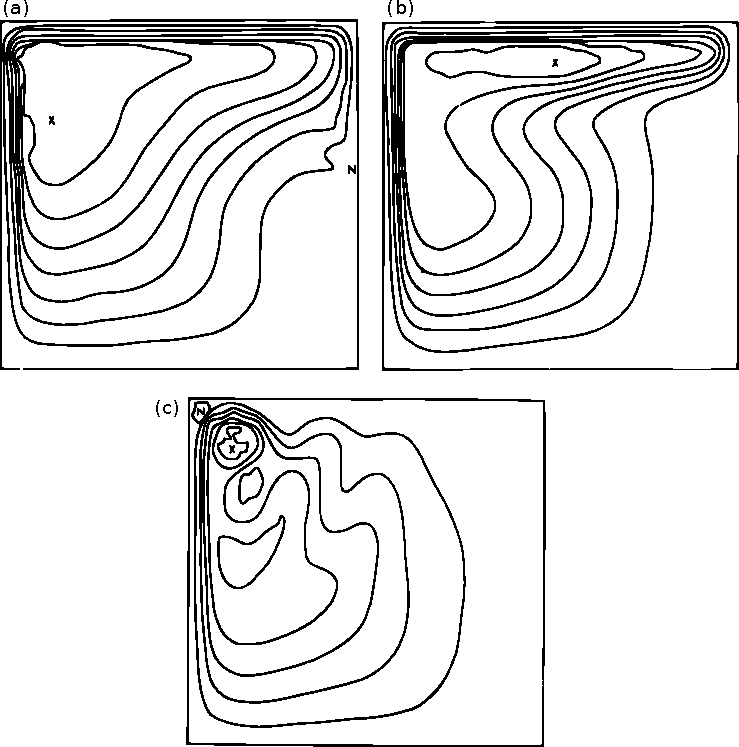
\includegraphics[width=.8\textwidth]{figures/physics/bc-blandford}
	\end{sidecaption}
\end{figure}

In computational fluid dynamics, a multitude of different lateral boundary conditions is used, each best suited for a specific range of physical problems. Probably the most popular boundary condition for flow tangential to a boundary is the \emph{no-slip} condition, which is motivated through a micro-scale picture of the flow: On a molecular level, fluid particles located immediately next to a wall tend to stick to it --- hence, the velocity shear between wall and fluid is enforced to be zero, \ie
%
\sidedef{No-Slip}{Boundary Condition}{%
\begin{equation}
\vec{u} \cdot \hat{t} = 0\quad \text{or} \quad \hat{n}\cdot\nabla\Psi = 0 \label{eq:noslip}
\end{equation}
}
%
with unit vectors \(\hat{t}\), \(\hat{n}\) tangential and normal to the boundary, respectively.

However, it is unclear why the argument of molecules sticking to a wall should apply to flow that is resolved at a scale of hundreds of kilometers. Boundary conditions that are frequently used in ocean modeling include the
\begin{items}
\item No-slip condition: \(\vec{u} \cdot \hat{t} = \hat{n}\cdot\nabla\Psi = 0\);
\item Free-slip condition: \(\zeta = \nabla^2 \Psi = 0\);
\item Superslip condition%
	\sidenote[-2]{When employing superslip or hyperslip conditions, the friction term may actually \emph{add} energy to the flow through the boundary (\cite{pedloskyoct}).}%
	: \(\hat{n} \cdot \nabla \zeta = 0\); and
\item Hyperslip condition: \(\hat{n} \cdot \nabla (\zeta + \beta y) = 0\).
\end{items}

Each of the described boundary conditions stems from a reasonable physical view of the interaction between wall and fluid \citep{pedloskyoct}. It is thus not possible to choose one particular of those boundary conditions \emph{a priori}, since neither is derived from first principles, and the boundary conditions in the real ocean are still unknown. The chosen boundary condition may impact the resulting circulation strongly (\figref{fig:bc-comparison}), and many numerical studies include simulations with several choices of boundary conditions (\eg \cite{killworth}).
\parabreak
Although the \enquote{correct} boundary condition is unknown, and although the transformation of vorticity in a boundary current \emph{is} sensitive to the chosen boundary condition (see \citebook{pedloskygfd}, Chapter 5), I will focus on the no-slip boundary condition in this thesis, since it is the only one that is deployed in \ac{CESM}.

\section{Friction and Viscosity}
\label{sec:physics-friction}
During the derivation of the ocean models described so far, frictional forces were intentionally left as general as possible (described through the unspecified term \(\vec{\mathcal{F}}\)). This was done because there simply is no unique answer to the question \emph{how this term should look like}. The two most popular formulations, a turbulent diffusion term and a bottom friction term, shall be introduced in the following sections (\secref{sec:friction-diff} and \secref{sec:bottom-friction}, respectively). Both of these terms are inherently over-simplifying the real processes, but often lead to a realistic picture of the ocean while allowing for analytical solutions of some simple special cases, which explains why they have become so popular.

After introducing these two formulations of friction, \secref{sec:cfl} and \secref{sec:noise} discuss some of the numerical aspects involved when solving diffusive \acp{PDE} (concerning numerical stability and noise, respectively).

\subsection{Turbulent Diffusion}
\label{sec:friction-diff}
The %
\marginelement{
\fancyquote{Lewis Fry Richardson}{%
	Big whirls have little whirls,\\That feed on their velocity;\\And little whirls have lesser whirls,\\And so on to viscosity.}%
}%
reason why a diffusive friction term \(\vec{\mathcal{F}} \sim A \nabla^2 \vec{u}\) is often chosen as a parameterization for lateral friction is \emph{not} because molecular diffusion is a particularly important process in the ocean --- in fact, it is in most cases negligible to a very high degree. The kinematic viscosity \(\nu\) of water is of the order of magnitude \(\SI{e-6}{\metre\squared\per\second}\), which, if \(\nu\) were the only contribution to the diffusivity \(A\), would imply that diffusive friction were utterly unimportant compared to other terms. However, it can be shown that unresolved turbulent motion can be modeled as a diffusive process: Turbulence creates mesoscale eddies with a typical size of \(\lesssim \SI{100}{\kilo\metre}\). Those eddies, superimposed on the mean flow, induce a velocity shear that acts to distribute momentum just like molecular diffusion, but several orders of magnitude stronger. A typical value for the \emph{turbulent diffusivity} \(A_H\) is \(\SI{e5}{\metre\squared\per\second} \gg \nu\). The derivation of the turbulent diffusion term is laid out in \citebook{pedloskygfd}, Chapter 4 --- here, we shall only sketch the most important ideas and assumptions going into it.
%
\begin{figure}
	\begin{sidecaption}[Turbulence in the ocean.]{Turbulence in the ocean. Snapshot of the ocean surface speed in an eddy-resolving model (effective resolution \ang{0.1}). Modeled with \ac{CESM} in a quasi-equilibrated control simulation. Note the widening effect of eddies on western boundary currents (\eg Gulf Stream and Kuroshio). Part of Mads Poulsen's PhD project.}[fig:eddy-resolving]
		\import{figures/physics/}{eddy-resolving.pdf_tex}
	\end{sidecaption}
\end{figure}

The starting point for the derivation of the turbulent diffusion term is the Reynolds decomposition: The flow field \(\vec{u}\) is decomposed into a mean flow, \(\mean{\vec{u}}\), and a (turbulent) small-scale flow, \(\vec{u}'\), such that\sidenote[-2]{It is already unclear whether this decomposition makes sense, \ie whether there exists an averaging time scale that is sufficiently short compared to the natural time scale of \(\mean{\vec{u}}\).}
%
\begin{equation}
\vec{u} = \mean{\vec{u}} + \vec{u}' \label{eq:reynolds-dec}
\end{equation}
%
which implies
%
\begin{equation}
\mean{\vec{u}} = \mean{\mean{\vec{u}}} + \mean{\vec{u'}} \rightarrow \mean{\vec{u'}} = 0.
\end{equation}
%
Inserting \eqref{eq:reynolds-dec} into the momentum equations, and identifying terms of the form \(\mean{u'v'}\) with the components of a stress tensor\sidenote[-1]{These stresses are consequently dubbed Reynolds-stresses.} \(\tau\), such that \eg
%
\begin{equation}
\mean{u'v'} = - \frac{\tau^{xy}}{\rho},
\end{equation}
%
leads to momentum equations of the form:\sidenote{Ddropping the averaging operators, \ie \(u \equiv \mean{u}\)}
%
\begin{equation}
u_t + (\vec{u}\cdot\nabla) u - fv = - \frac{1}{\rho} p_x + \frac{1}{\rho} \left( \tau^{xx}_x + \tau^{xy}_y + \tau^{xz}_z \right) + \nu \nabla^2 u.
\label{eq:stressmomentum}
\end{equation}
%
This formulation of the momentum equations still contains the unknown stresses (in terms of the mean flow) \(\tau^{ij}\). Finding a formulation for \(\tau\) that depends on the mean flow \(\vec{u}\) only is called the \emph{closure problem}, and is highly non-trivial \citep{pedloskygfd}. A simple (but crude) closure is obtained by assuming that the stress acting on the fluid depends linearly on the shear of the velocity field, such that
%
\begin{equation}
\tau^{ij} = \rho \left( A^i (\hat{j} \cdot \vec{u})_i + A^j (\hat{i} \cdot \vec{u})_j \right).
\end{equation}
%
Then, the stress terms in the momentum equation for \(u\) \eqref{eq:stressmomentum} become
%
\begin{equation}
\frac{1}{\rho} \bigl( \tau^{xx}_x + \tau^{xy}_y + \tau^{xz}_z \bigr) = \bigl(A^x u_x\bigr)_x + \bigl(A^y u_y\bigr)_y + \bigl(A^z u_z\bigr)_z,
\end{equation}
%
and analogous formulations are found for the other components of the momentum equation. In the special case of constant diffusion coefficients \(A^x(x,y,z) \equiv A^y(x,y,z) \equiv A_H\) and \(A^z \equiv 0\), this reduces to the well-known form of lateral diffusive friction:
%
\begin{equation}
\vec{\mathcal{F}} = A_H \nabla_H^2 \vec{u}.
\end{equation}
%
Another important reason why this simple solution of the closure problem is widely used in Oceanography is a practical one: A friction term depending on the curvature of the flow field (\ie \(\nabla^2 \vec{u}\)) acts to reduce numerical errors present in most implementations: many discretizations of the momentum \acp{PDE} introduce noise on a scale of one grid spacing \(\updel x\). This small-scale noise inherently leads to a large curvature of the flow, which is effectively dissipated by diffusive friction. It is thus usually desirable to include a diffusive term into the model equations (\cf \secref{sec:noise}).

Because \(A_H\) is determined by unresolved small-scale motion, this formulation depends on the model resolution at hand. In eddy-resolving models (that, on a global scale, can only be ran at the World's largest super computers), \(A_H\) can be chosen extremely small, as the effects of turbulence on the mean flow are modeled directly through the nonlinear terms of the small-scale flow (such as \eg \(u'v'\)). Those high-resolution models with a spatial scale of \(\lesssim \SI{20}{\kilo\metre}\) reveal the true turbulent nature of the ocean (\figref{fig:eddy-resolving}).

\subsection{Bottom Friction}
\label{sec:bottom-friction}
In his ground-breaking paper, \citeauthorfull{stommel} was the first to tie the observed westward intensification of the ocean circulation to the Earth's planetary vorticity gradient \citep{stommel}, just like \citeauthorfull{munk} did several years later \citep{munk}. The western boundary current solution Stommel presented is different from the Munk solution in that it uses different friction term: Instead of including a diffusive lateral friction model, Stommel introduced a mathematically much simpler Rayleigh friction term acting to dissipate momentum directly:
%
\begin{equation}
\vec{\mathcal{F}} = - \kappa \vec{u}. \label{eq:rayleigh-friction}
\end{equation}
%
Though seemingly highly artificial, this term can be motivated in the framework of boundary layer theory. Considering a frictional boundary layer (Ekman layer) at the bottom of the ocean, it can be derived that the frictional drag acting on the interior flow creates a vertical motion, which in turn leads to a Rayleigh dissipation term like \eqref{eq:rayleigh-friction} to leading order, as laid out in \citebook{pedloskygfd}.

Many authors decide to introduce friction into their model via a bottom friction term alone (\eg \cite{kawase}), and the question whether bottom or lateral friction is dominant in the ocean is still unanswered. Bottom friction is present in \ac{POP2} and thus \ac{CESM}, but is playing a minor role compared to lateral friction.

\subsection{Stability Conditions}
\label{sec:cfl}
When %
\marginelement{Considerations in this section follow Chapters 4, 5 \oldand 6 of \citetitle{wesselingcfd} by \citeauthorfull{wesselingcfd} \citep{wesselingcfd}.}%
solving a system of non-stationary advection-diffusion equations (such as the nonlinear and friction terms in the momentum equations \eqref{eq:momentumvec}), \ie 
%
\begin{equation}
\vec*{u}{t} + \underbrace{(\vec{u}\cdot\nabla)\vec{u} - A \nabla^2 \vec{u}}_{\mathcal{L}\vec{u}} = 0
\end{equation}
%
it is usually transformed into a system of \acp{ODE} by discretizing the spatial part of the \ac{PDE} (in form of the spatial operator \(\mathcal{L}\)) into a discrete operator \(\mathcal{L}_h\):
%
\begin{equation}
(\vec*{u}{h})_t = - \mathcal{L}_h(\vec*{u}{h}) \vec*{u}{h}. \label{eq:spatial-discrete}
\end{equation}
%
where \(\vec*{u}{h}\) just denotes a discrete version of the continuous velocity \(\vec{u}\). In \eqref{eq:spatial-discrete}, \(\mathcal{L}_h\) depends on \(\vec*{u}{h}\) due to the advection term \((\vec{u}\cdot\nabla)\vec{u}\). However, although unproven in the general case, it is usually conjectured that a discretization of the nonlinear term is stable if and only if the method is stable for an operator that only depends on a \enquote{frozen} value of \(u\) (see \eg \cite{chorin}), \ie if \(\vec*{u}{h} = - \mathcal{L}_h(\vec*{u}{h}^*)\vec*{u}{h}\) is stable. The stability analysis is thus carried out for a convection-diffusion problem, and assumed to hold for the advection-diffusion equations as well. Using an explicit \emph{finite difference scheme}\sidenote[-4]{Implicit schemes are also possible, and usually lead to a much larger stability region, but they come with an additional computational cost for solving a linear system in every time step.}, \(\mathcal{L}_h\) becomes:
%
\begin{equation}
\updel t \mathcal{L}_h = \sum_i \Bigg[ \underbrace{\frac{|\hat{i} \cdot \vec*{u}{h}^*| \updel t}{\updel x_i}}_{c_i} \Gamma_i(\vec*{u}{h}) + \underbrace{\frac{2A\updel t}{(\updel x_i)^2}}_{d_i} \Lambda_i(\vec*{u}{h}) \Bigg]
\end{equation}
%
with
%
\begin{items}
\item A sum over all coordinates \(i\) (in this case, \(i\) corresponds to \(x\),\(y\),\(z\));
\item Time step size \(\updel t\);
\item Mesh sizes \(\updel x_i\);
\item Discretizations for the convection and diffusion terms, \(\Gamma\) and \(\Lambda\), respectively. Simple (but bad) formulations for these terms would be\sidenote[-1]{More sophisticated discretizations such as upwinding or \(\kappa\)-schemes are given in \cite{wesselingcfd}.}
	%
	\begin{gather}
	\Gamma_i \vec*{u}{h} = u_i^{j+1} - u_i^{j} \\
	\text{and} \\
	\Lambda_i \vec*{u}{h} = \frac{1}{2} u_i^{j-1} - u^j + \frac{1}{2} u_i^{j+1}
	\end{gather}
	%
	with \(u_i \equiv \hat{i}\cdot\vec*{u}{h}\) and assuming \(u_i > 0\).
\end{items}
%
The dimensionless parameters \(c_i\) are called \emph{CFL numbers}, and were first introduced in \cite{cfl}. \(d_i\) are sometimes called diffusion numbers, or diffusive CFL numbers.

A stability condition for the resulting \ac{ODE} can then be obtained using \eg von Neumann analysis, and depends on the chosen discretization of the time derivative, \((u_h)_t\). \citet{wesselingcfd} derives stability criteria for several popular time discretization schemes, which all relate \(c_i\) and \(d_i\) to constant values. For a second order central difference scheme in space and explicit Euler in time, one obtains the following necessary and sufficient conditions for stability:
%
\sidedef{CFL condition}{}{
\begin{equation}
\sum_i \frac{c_i^2}{d_i} \leq 1 \label{eq:cfl}
\end{equation}
}
%
and
%
\sidedef{Viscous CFL condition}{}{
\begin{equation}
\sum_i d_i \leq 1. \label{eq:diffcfl}
\end{equation}
}

Since in \ac{CESM} both \(\updel x_i\) and \(\updel t\) are fixed, \eqref{eq:diffcfl} leads to a condition for the viscosity \(A\):\sidenote[-1]{As given in the \ac{POP2} manual, \cite{pop2}.}
%
\begin{equation}
A \leq A_\text{cfl} = \frac{\updel x^2 + \updel y^2}{4 \updel t} \label{eq:cflcesm}
\end{equation} 
%
This limits the values of viscosity that can be used during the model runs in \chapref{chap:cesm-runs}.

\subsection{Numerical Noise}
\label{sec:noise}
\begin{figure}
	\begin{sidecaption}[The generation of numerical noise in a shallow-water model without lateral friction.]{The generation of numerical noise in a shallow-water model without lateral friction. Note the jagged edges along the boundaries. Bottom figure shows the reduction of noise in the same data averaged with a boxcar filter.}[fig:checkerboard]
	\antimpjustification
	\importpgf{figures/physics/checkerboard/}{checkerboard.pgf}
	\end{sidecaption}
\end{figure}
There are several processes that may introduce artificial dispersive noise into the numerical solution of a differential equation. The most straightforward way to see how this happens is by considering central finite differences, such as
%
\begin{equation}
\left. \frac{\partial f}{\partial x} \right|_{x_i} \approx \frac{f(x_{i+1}) - f(x_{i-1})}{x_{i+1} - x_{i-i}}
\end{equation}
%
as an approximation of the gradient of a function \(f\) in \(x\)-direction. This scheme connects the value of \(f\) at a point \(x_i\) with the values at \(x_{i+1}\) and \(x_{i-1}\) alone. This means that grid points at even and odd \(i\) may decouple in the steady state, creating an alternating pattern in the solution (sometimes referred to as \emph{checkerboard effect}). Since the pressure and nonlinear terms in the momentum equations both involve a first derivative in space, this effect can also be observed in many ocean simulations when these terms become dominant.

One important feature of this type of noise is that it occurs on \emph{grid scale}. This allows us to quantify and filter dispersive noise, \eg by averaging over adjacent grid cells (\figref{fig:checkerboard}), as in \cite{jochum}.

\section{Global Ocean Currents}
\label{sec:physics-currents}
This section presents some of the features of the \emph{observed} ocean circulation (in contrast and comparison to the theoretical findings described in \secref{sec:physics-solutions}). Since the focus of my thesis lies on the global-scale ocean circulation (the \ac{MOC}), a description of the gyre circulations, which are mostly in Sverdrup balance (\secref{sec:sverdrup}), is being omitted.

First up, the global features of the \ac{MOC} as a whole are presented, followed by a more detailed examination of some local regions of interest like the \ac{AMOC} and the \ac{ITF}.

\begin{figure}
	\begin{whole}
		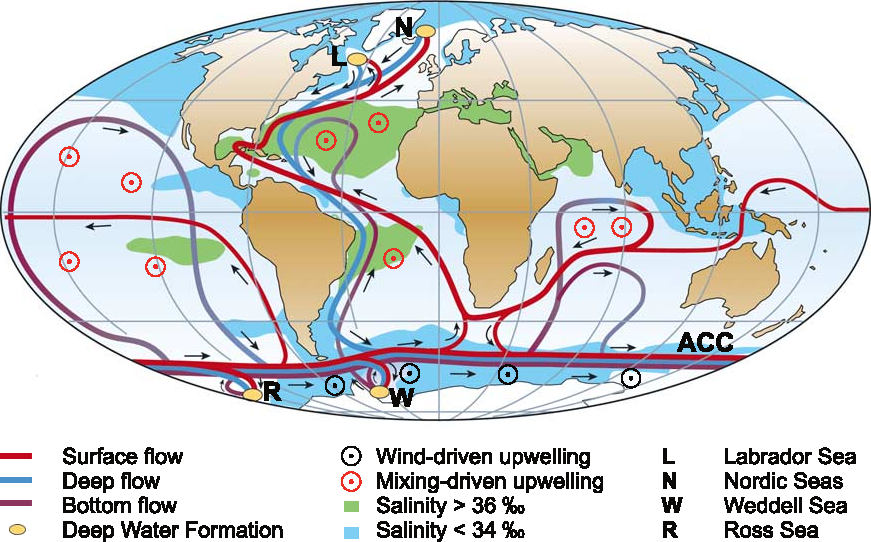
\includegraphics[width=.8\linewidth]{physics/kuhlbrodt}
	\end{whole}
	\caption{The \ac{MOC}. From \cite{kuhlbrodt}, after \cite{rahmstorf}.}
	\label{fig:kuhlbrodt-moc}
\end{figure}

\subsection{The \acf{MOC}}
The%
\sidefigure[One of the first illustrations of the \ac{MOC}.]{One of the first illustrations of the \ac{MOC}. \cite{broecker}. \label{fig:boecker-moc}}{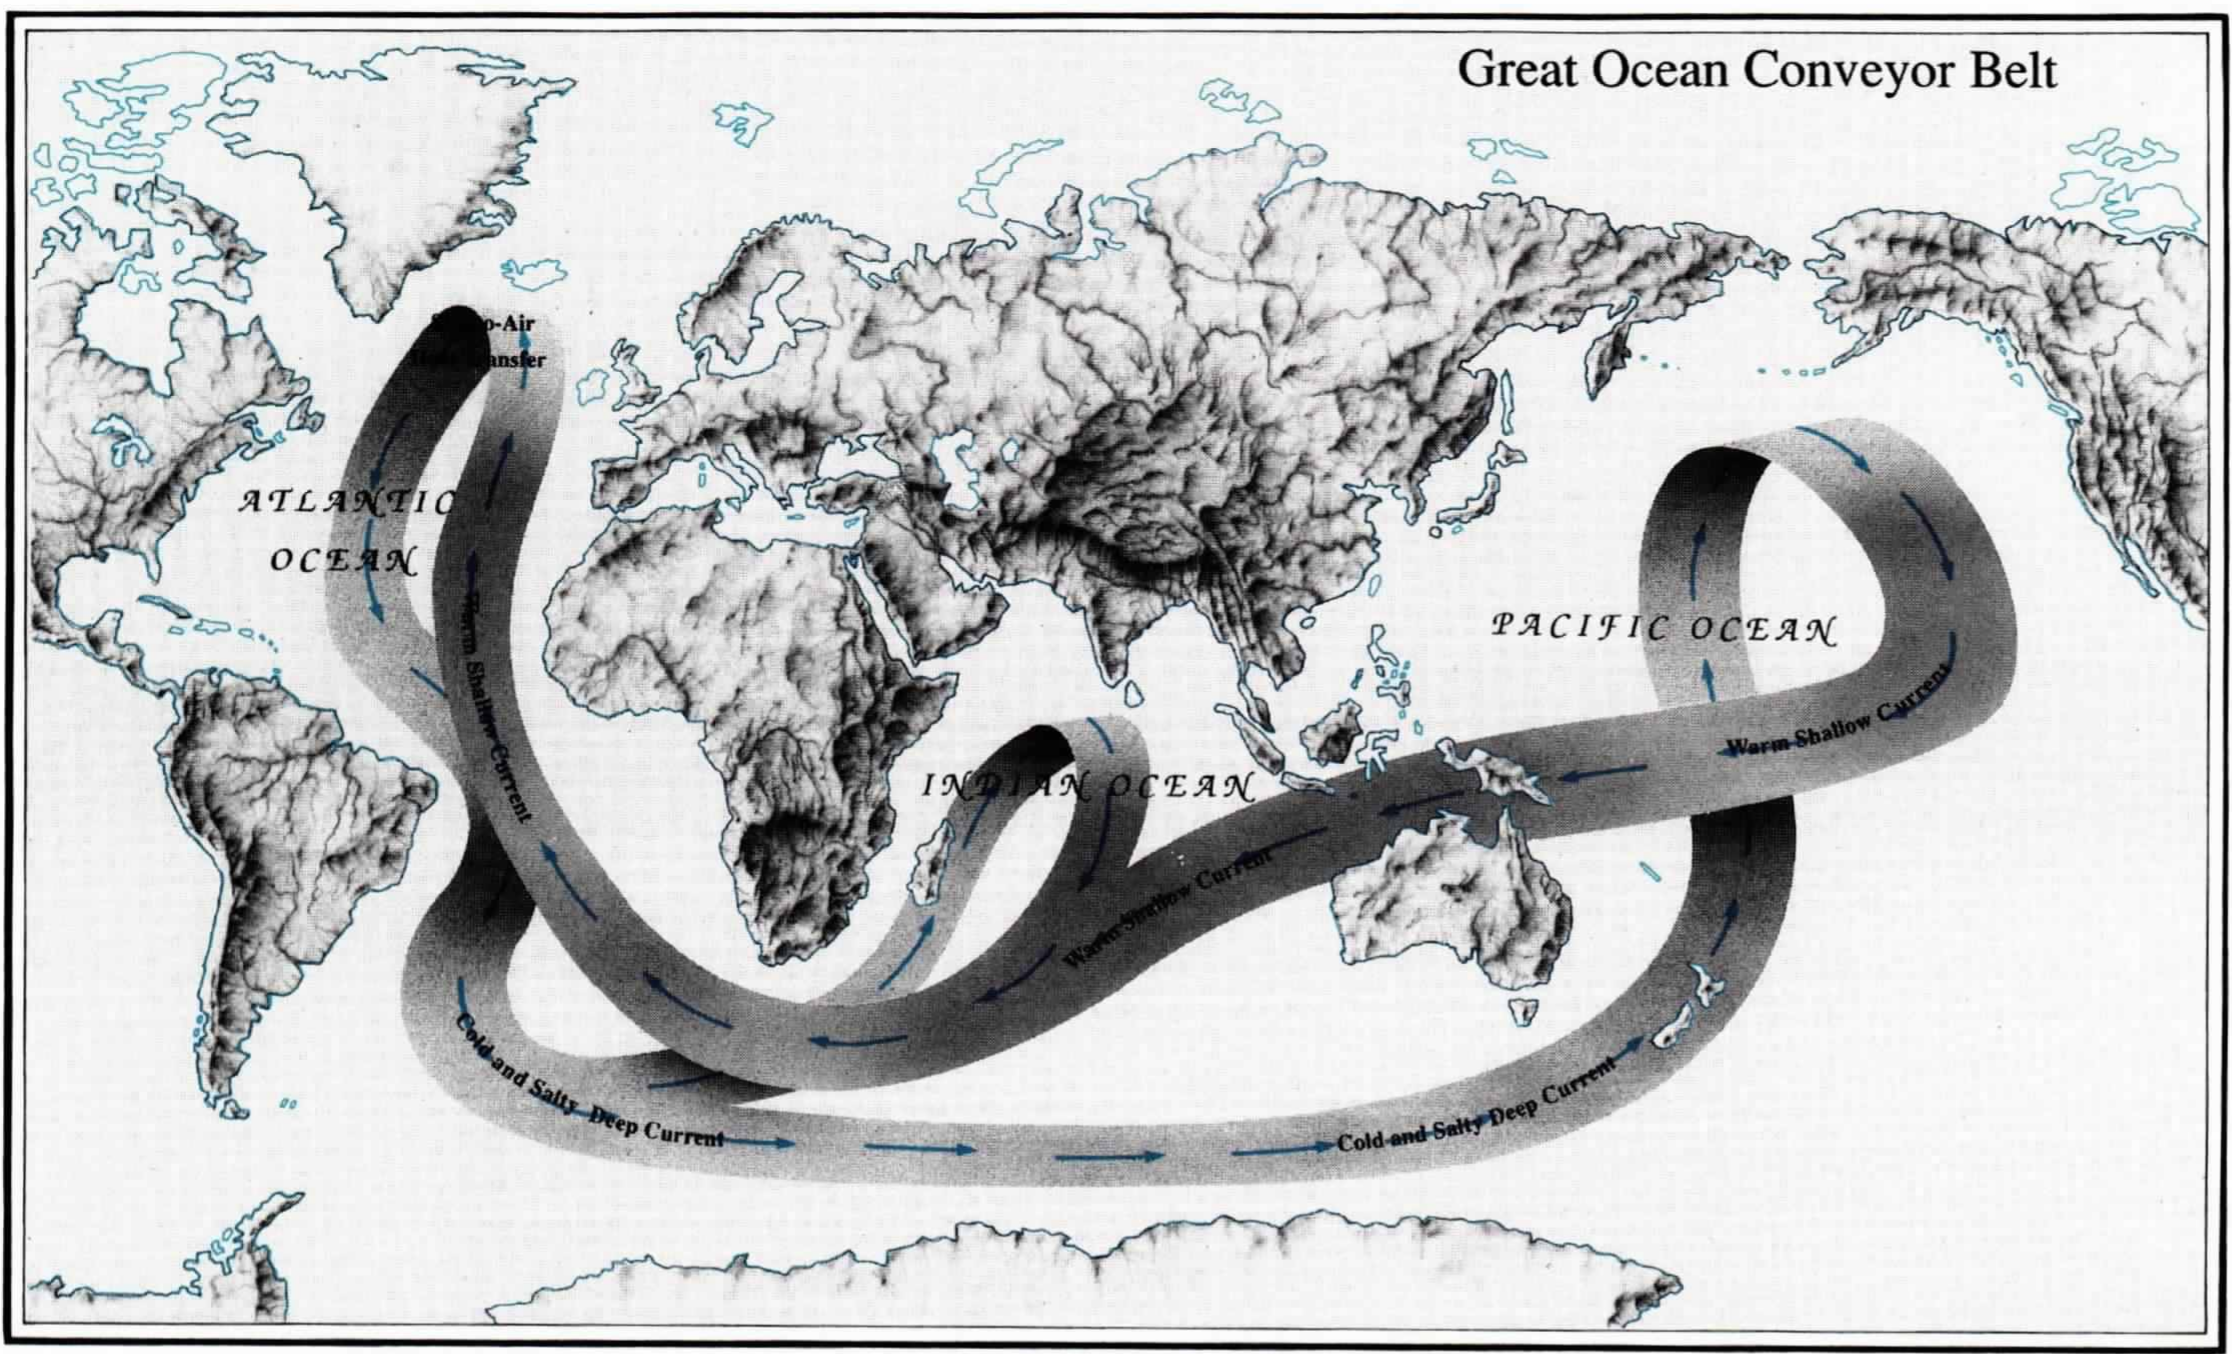
\includegraphics[width=.9\marginparwidth]{physics/boecker-moc}}[-2]%
idea of the \ac{MOC} as a great global \enquote{conveyor belt} that connects water masses all around the world has inspired many generations of oceanographers: Parts of the \ac{MOC} were described as early as the first half of the \num{20}\textsuperscript{th} century, \eg in \cite{wuest}. The pathway of this conveyor belt has often been illustrated --- one early, though quite simplified, depiction was done by \citeauthor{broecker} for the \work{Natural History} magazine (\figref{fig:boecker-moc}), which in term became a logo for the \work{Global Change Research Initiative} (see \cite{broecker}).

A more modern, and more accurate depiction of the \ac{MOC} is found in \cite{kuhlbrodt} (\figref{fig:kuhlbrodt-moc}). This illustration correctly emphasizes the role of the Southern Ocean in distributing water masses between the world's oceans\sidenote[-2]{Note that only the density-driven thermohaline circulation is shown in these illustrations --- flow in Sverdrup balance such as the gyre circulations are omitted.}. The crucial role of the Southern Ocean is also stressed in \cite{marshall}.

In the \ac{MOC}, deep water created in the North Atlantic flows all the way south and joins the \ac{ACC}. In this region, strong wind-driven upwelling eventually causes this water to emerge. Then, it flows northward along one of the boundaries in the ocean (along the shore of Africa, South America, or Australia). Flow in the Atlantic then joins the \ac{AMOC} (see below), while there is no similar deeply penetrating overturning circulation in the Pacific. In the Pacific, large parts of the flow from the Southern Ocean end up in zonal jets like the \ac{NEC}, which returns water to the southern hemisphere mainly via the \ac{ITF}.

The exact driving forces of the \ac{MOC} and their relative importances are still largely unclear. \citeauthor{kuhlbrodt} suggest that, at least in the \ac{AMOC}, both wind-driven and mixing-driven upwelling are crucial driving processes of the overturning.

\subsection{Local Features}
\subsubsection{The \acf{AMOC}}
The%
\sidefigure{Vertical stream function of the \ac{AMOC} in the \ac{CESM} \grid{x3} default run.}[fig:amoc-default]%
{\importpgf{figures/physics/amoc-default/}{amoc-default.pgf}}%
%
branch of the \ac{MOC} that distributes water in the Atlantic all the way between the Southern Ocean and the Arctic is known as the \ac{AMOC}. A great overview of the \ac{AMOC} and the processes that control it is given in \cite{kuhlbrodt}. In their introduction, they state:

\q{\slshape%
	The deep Atlantic meridional overturning circulation
	(AMOC) consists of four main branches: upwelling processes that transport volume from depth to near the ocean
	surface, surface currents that transport relatively light water
	toward high latitudes, deep-water formation regions where
	waters become denser and sink, and deep currents closing
	the loop. These four branches span the entire Atlantic on
	both hemispheres, forming a circulation system that consists
	of two overturning cells, a deep one with North Atlantic
	Deep Water (NADW) and an abyssal one with Antarctic
	Bottom Water (AABW).
}

These features of the \ac{AMOC} are also present in the numerical \ac{CESM} simulations (\figref{fig:amoc-default}). Roughly \SI{12}{\sv} of water entering the Atlantic between the surface and a depth of about \SI{1200}{\metre} is flowing northward, some of it upwelling at the equator, until high latitudes are reached. There, it is converted to \ac{NADW}, sinking to a depth of about \num{1.4} to \SI{3.0}{\kilo\metre}. This deep branch of the \ac{AMOC} proceeds southward, all the way to the Southern Ocean, where the circulation is closed (not shown).

The second, abyssal overturning cell is located at depths of \(\gtrsim \SI{3}{\kilo\metre}\), but carries only a weak transport compared to the upper cell (\SI{2}{\sv} in the \ac{CESM} \ang{3} default run), and is not examined in this thesis.

\subsubsection{Indonesian Throughflow}
The \acf{ITF} is the main pathway for water originating in the Southern Ocean from the Northern Pacific to the Indian Ocean, and thus back to the southern hemisphere, closing the overturning in the Pacific (mean transport of about \SI{15}{\sv}, \cite{sprintall}). Due to its complex pathway between the Indonesian islands, the \ac{ITF} is sensitive to changes in geometry (\cite{jochumind}), and thus might also be influenced by changes in viscosity.

The \ac{ITF} is located right at the point where two boundary currents\sidenote{The \ac{MC} from the north and the \ac{NGCUC} from the south, which carries water from the \ac{SEC}.} turn eastward between the islands of Mindanao, Halmahera, and Papua, feeding the \ac{NECC} (\figref{fig:itf-currents}). In the retroflection regions, semi\hyp{}permanent eddies form, the Mindanao and Halmahera eddies. From the Pacific Ocean, the \ac{ITF} leads through either the Makassar Strait between Kalimantan and Sulawesi, or the Lifamatola Passage east of that.

\begin{figure}
	\centering
	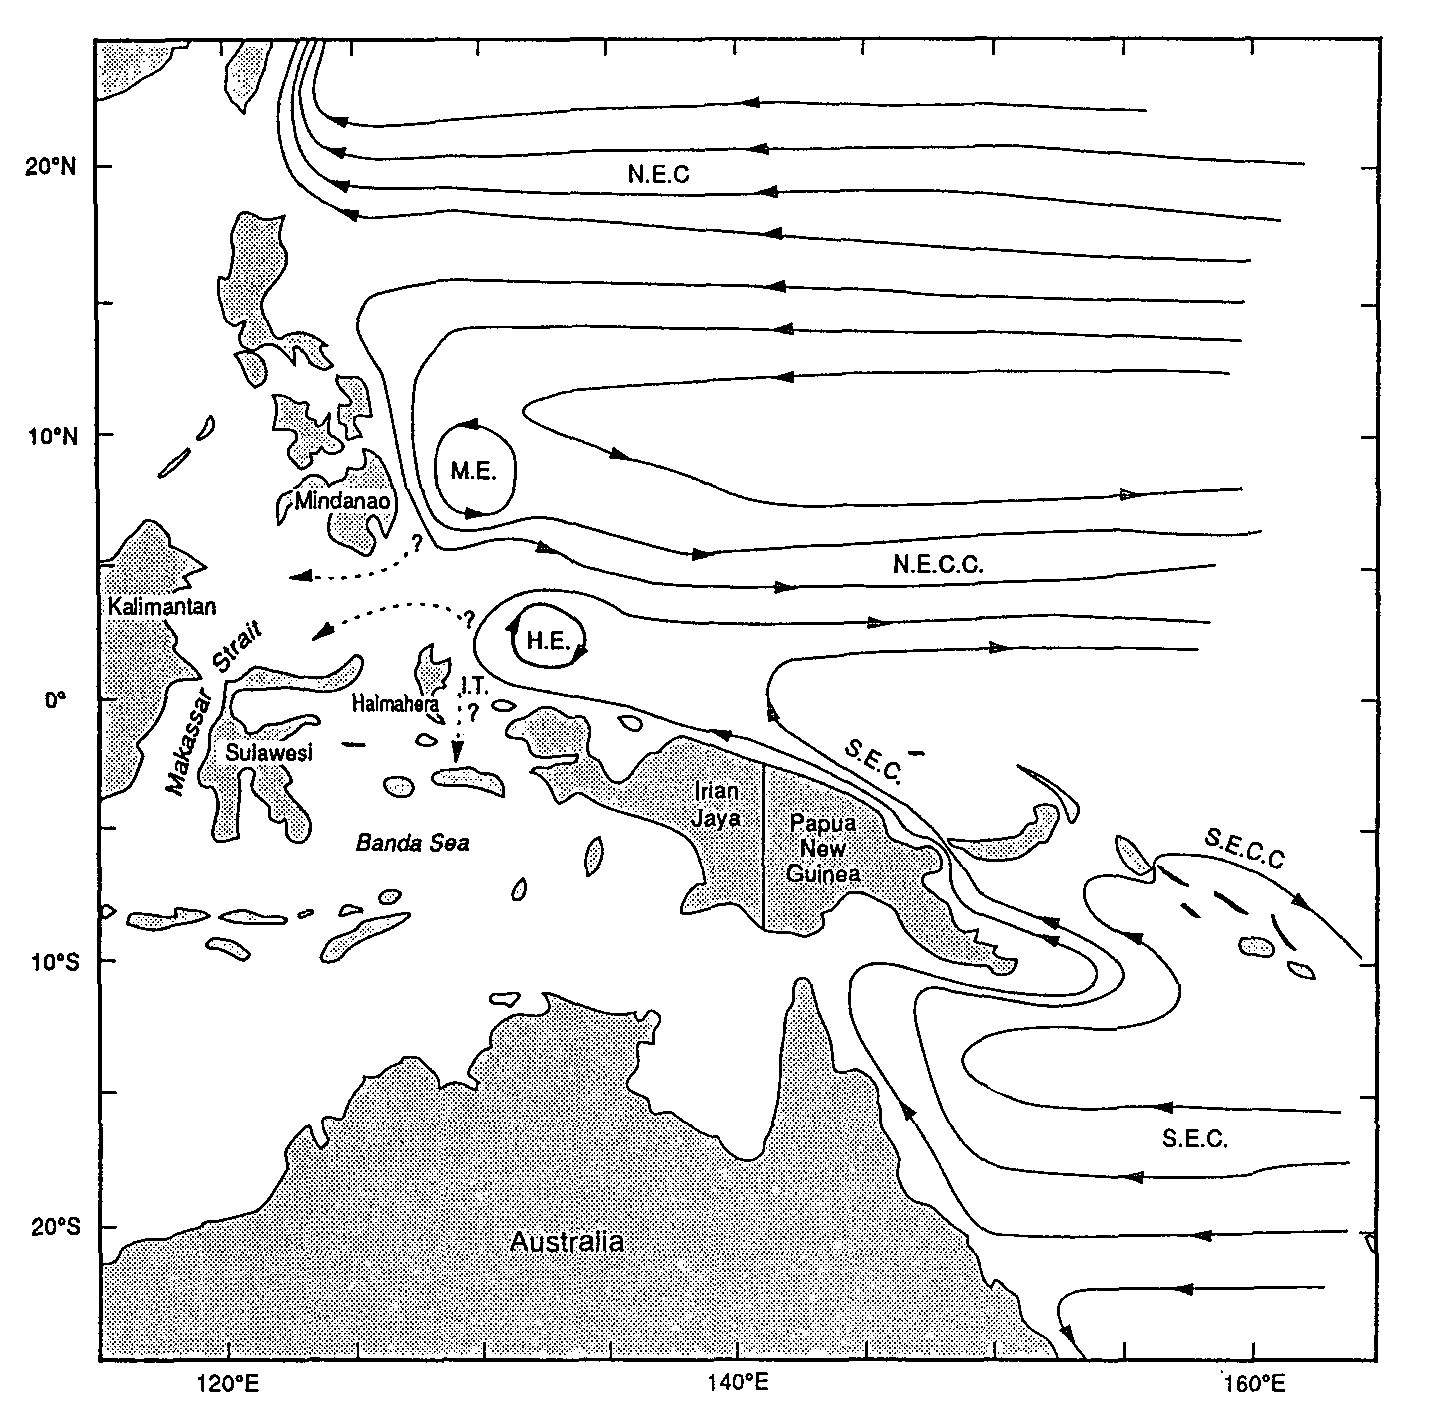
\includegraphics[width=.85\linewidth]{physics/itf}
	\caption[Currents in the \ac{ITF}-region.]{Currents in the \ac{ITF}-region. After \cite{godfreyind}. Note that Irian Jaya is officially called (West) Papua since 2002.}
	\label{fig:itf-currents}
\end{figure}